\documentclass[]{book}
\usepackage{lmodern}
\usepackage{amssymb,amsmath}
\usepackage{ifxetex,ifluatex}
\usepackage{fixltx2e} % provides \textsubscript
\ifnum 0\ifxetex 1\fi\ifluatex 1\fi=0 % if pdftex
  \usepackage[T1]{fontenc}
  \usepackage[utf8]{inputenc}
\else % if luatex or xelatex
  \ifxetex
    \usepackage{mathspec}
  \else
    \usepackage{fontspec}
  \fi
  \defaultfontfeatures{Ligatures=TeX,Scale=MatchLowercase}
\fi
% use upquote if available, for straight quotes in verbatim environments
\IfFileExists{upquote.sty}{\usepackage{upquote}}{}
% use microtype if available
\IfFileExists{microtype.sty}{%
\usepackage{microtype}
\UseMicrotypeSet[protrusion]{basicmath} % disable protrusion for tt fonts
}{}
\usepackage[margin=1in]{geometry}
\usepackage{hyperref}
\hypersetup{unicode=true,
            pdftitle={A Minimal ML Example},
            pdfauthor={M-Team},
            pdfborder={0 0 0},
            breaklinks=true}
\urlstyle{same}  % don't use monospace font for urls
\usepackage{natbib}
\bibliographystyle{apalike}
\usepackage{color}
\usepackage{fancyvrb}
\newcommand{\VerbBar}{|}
\newcommand{\VERB}{\Verb[commandchars=\\\{\}]}
\DefineVerbatimEnvironment{Highlighting}{Verbatim}{commandchars=\\\{\}}
% Add ',fontsize=\small' for more characters per line
\usepackage{framed}
\definecolor{shadecolor}{RGB}{248,248,248}
\newenvironment{Shaded}{\begin{snugshade}}{\end{snugshade}}
\newcommand{\KeywordTok}[1]{\textcolor[rgb]{0.13,0.29,0.53}{\textbf{#1}}}
\newcommand{\DataTypeTok}[1]{\textcolor[rgb]{0.13,0.29,0.53}{#1}}
\newcommand{\DecValTok}[1]{\textcolor[rgb]{0.00,0.00,0.81}{#1}}
\newcommand{\BaseNTok}[1]{\textcolor[rgb]{0.00,0.00,0.81}{#1}}
\newcommand{\FloatTok}[1]{\textcolor[rgb]{0.00,0.00,0.81}{#1}}
\newcommand{\ConstantTok}[1]{\textcolor[rgb]{0.00,0.00,0.00}{#1}}
\newcommand{\CharTok}[1]{\textcolor[rgb]{0.31,0.60,0.02}{#1}}
\newcommand{\SpecialCharTok}[1]{\textcolor[rgb]{0.00,0.00,0.00}{#1}}
\newcommand{\StringTok}[1]{\textcolor[rgb]{0.31,0.60,0.02}{#1}}
\newcommand{\VerbatimStringTok}[1]{\textcolor[rgb]{0.31,0.60,0.02}{#1}}
\newcommand{\SpecialStringTok}[1]{\textcolor[rgb]{0.31,0.60,0.02}{#1}}
\newcommand{\ImportTok}[1]{#1}
\newcommand{\CommentTok}[1]{\textcolor[rgb]{0.56,0.35,0.01}{\textit{#1}}}
\newcommand{\DocumentationTok}[1]{\textcolor[rgb]{0.56,0.35,0.01}{\textbf{\textit{#1}}}}
\newcommand{\AnnotationTok}[1]{\textcolor[rgb]{0.56,0.35,0.01}{\textbf{\textit{#1}}}}
\newcommand{\CommentVarTok}[1]{\textcolor[rgb]{0.56,0.35,0.01}{\textbf{\textit{#1}}}}
\newcommand{\OtherTok}[1]{\textcolor[rgb]{0.56,0.35,0.01}{#1}}
\newcommand{\FunctionTok}[1]{\textcolor[rgb]{0.00,0.00,0.00}{#1}}
\newcommand{\VariableTok}[1]{\textcolor[rgb]{0.00,0.00,0.00}{#1}}
\newcommand{\ControlFlowTok}[1]{\textcolor[rgb]{0.13,0.29,0.53}{\textbf{#1}}}
\newcommand{\OperatorTok}[1]{\textcolor[rgb]{0.81,0.36,0.00}{\textbf{#1}}}
\newcommand{\BuiltInTok}[1]{#1}
\newcommand{\ExtensionTok}[1]{#1}
\newcommand{\PreprocessorTok}[1]{\textcolor[rgb]{0.56,0.35,0.01}{\textit{#1}}}
\newcommand{\AttributeTok}[1]{\textcolor[rgb]{0.77,0.63,0.00}{#1}}
\newcommand{\RegionMarkerTok}[1]{#1}
\newcommand{\InformationTok}[1]{\textcolor[rgb]{0.56,0.35,0.01}{\textbf{\textit{#1}}}}
\newcommand{\WarningTok}[1]{\textcolor[rgb]{0.56,0.35,0.01}{\textbf{\textit{#1}}}}
\newcommand{\AlertTok}[1]{\textcolor[rgb]{0.94,0.16,0.16}{#1}}
\newcommand{\ErrorTok}[1]{\textcolor[rgb]{0.64,0.00,0.00}{\textbf{#1}}}
\newcommand{\NormalTok}[1]{#1}
\usepackage{longtable,booktabs}
\usepackage{graphicx,grffile}
\makeatletter
\def\maxwidth{\ifdim\Gin@nat@width>\linewidth\linewidth\else\Gin@nat@width\fi}
\def\maxheight{\ifdim\Gin@nat@height>\textheight\textheight\else\Gin@nat@height\fi}
\makeatother
% Scale images if necessary, so that they will not overflow the page
% margins by default, and it is still possible to overwrite the defaults
% using explicit options in \includegraphics[width, height, ...]{}
\setkeys{Gin}{width=\maxwidth,height=\maxheight,keepaspectratio}
\IfFileExists{parskip.sty}{%
\usepackage{parskip}
}{% else
\setlength{\parindent}{0pt}
\setlength{\parskip}{6pt plus 2pt minus 1pt}
}
\setlength{\emergencystretch}{3em}  % prevent overfull lines
\providecommand{\tightlist}{%
  \setlength{\itemsep}{0pt}\setlength{\parskip}{0pt}}
\setcounter{secnumdepth}{5}
% Redefines (sub)paragraphs to behave more like sections
\ifx\paragraph\undefined\else
\let\oldparagraph\paragraph
\renewcommand{\paragraph}[1]{\oldparagraph{#1}\mbox{}}
\fi
\ifx\subparagraph\undefined\else
\let\oldsubparagraph\subparagraph
\renewcommand{\subparagraph}[1]{\oldsubparagraph{#1}\mbox{}}
\fi

%%% Use protect on footnotes to avoid problems with footnotes in titles
\let\rmarkdownfootnote\footnote%
\def\footnote{\protect\rmarkdownfootnote}

%%% Change title format to be more compact
\usepackage{titling}

% Create subtitle command for use in maketitle
\newcommand{\subtitle}[1]{
  \posttitle{
    \begin{center}\large#1\end{center}
    }
}

\setlength{\droptitle}{-2em}

  \title{A Minimal ML Example}
    \pretitle{\vspace{\droptitle}\centering\huge}
  \posttitle{\par}
    \author{M-Team}
    \preauthor{\centering\large\emph}
  \postauthor{\par}
      \predate{\centering\large\emph}
  \postdate{\par}
    \date{2019-03-04}

\usepackage{booktabs}

\begin{document}
\maketitle

{
\setcounter{tocdepth}{1}
\tableofcontents
}
\hypertarget{basic-tutorial}{%
\chapter{Basic tutorial}\label{basic-tutorial}}

\begin{figure}
\centering
\includegraphics{https://m-clark.github.io/introduction-to-machine-learning/preface.html}
\caption{m-clark ML}
\end{figure}

\#Regularized Regression

\begin{Shaded}
\begin{Highlighting}[]
\NormalTok{wine <-}\StringTok{ }\KeywordTok{read.csv}\NormalTok{(}\StringTok{"~/Dropbox/M-Team/ML/wine.csv"}\NormalTok{)}
\KeywordTok{str}\NormalTok{(wine)}
\end{Highlighting}
\end{Shaded}

\begin{verbatim}
## 'data.frame':    6497 obs. of  15 variables:
##  $ X                   : int  0 1 2 3 4 5 6 7 8 9 ...
##  $ fixed.acidity       : num  7.4 7.8 7.8 11.2 7.4 7.4 7.9 7.3 7.8 7.5 ...
##  $ volatile.acidity    : num  0.7 0.88 0.76 0.28 0.7 0.66 0.6 0.65 0.58 0.5 ...
##  $ citric.acid         : num  0 0 0.04 0.56 0 0 0.06 0 0.02 0.36 ...
##  $ residual.sugar      : num  1.9 2.6 2.3 1.9 1.9 1.8 1.6 1.2 2 6.1 ...
##  $ chlorides           : num  0.076 0.098 0.092 0.075 0.076 0.075 0.069 0.065 0.073 0.071 ...
##  $ free.sulfur.dioxide : num  11 25 15 17 11 13 15 15 9 17 ...
##  $ total.sulfur.dioxide: num  34 67 54 60 34 40 59 21 18 102 ...
##  $ density             : num  0.998 0.997 0.997 0.998 0.998 ...
##  $ pH                  : num  3.51 3.2 3.26 3.16 3.51 3.51 3.3 3.39 3.36 3.35 ...
##  $ sulphates           : num  0.56 0.68 0.65 0.58 0.56 0.56 0.46 0.47 0.57 0.8 ...
##  $ alcohol             : num  9.4 9.8 9.8 9.8 9.4 9.4 9.4 10 9.5 10.5 ...
##  $ quality             : Factor w/ 2 levels "bad","good": 1 1 1 2 1 1 1 2 2 1 ...
##  $ color               : Factor w/ 2 levels "red","white": 1 1 1 1 1 1 1 1 1 1 ...
##  $ white               : int  0 0 0 0 0 0 0 0 0 0 ...
\end{verbatim}

\begin{Shaded}
\begin{Highlighting}[]
\KeywordTok{library}\NormalTok{(caret)}
\KeywordTok{library}\NormalTok{(tidyverse)}
\KeywordTok{library}\NormalTok{(glmnet)}
\KeywordTok{library}\NormalTok{(class)}
\KeywordTok{library}\NormalTok{(randomForest)}
\KeywordTok{library}\NormalTok{(e1071)}
\KeywordTok{library}\NormalTok{(ggplot2)}
\end{Highlighting}
\end{Shaded}

\hypertarget{regularized-regression}{%
\chapter{Regularized Regression}\label{regularized-regression}}

\begin{Shaded}
\begin{Highlighting}[]
\KeywordTok{set.seed}\NormalTok{(}\DecValTok{1234}\NormalTok{) }\CommentTok{# so that the indices will be the same when re-run}
\CommentTok{# 抽出80%樣本來train, output format is matrix}
\NormalTok{trainIndices =}\StringTok{ }\KeywordTok{createDataPartition}\NormalTok{(wine}\OperatorTok{$}\NormalTok{quality, }\DataTypeTok{p=}\NormalTok{.}\DecValTok{8}\NormalTok{, }\DataTypeTok{list=}\NormalTok{F) }

\CommentTok{# delete highly correlated free.sulfur and density}
\NormalTok{wine_train =}\StringTok{ }\NormalTok{wine }\OperatorTok\StringTok{ }
\StringTok{  }\KeywordTok{select}\NormalTok{(}\OperatorTok{-}\NormalTok{free.sulfur.dioxide, }\OperatorTok{-}\NormalTok{density, }\OperatorTok{-}\NormalTok{color, }\OperatorTok{-}\NormalTok{white) }\OperatorTok\StringTok{ }
\StringTok{  }\KeywordTok{slice}\NormalTok{(trainIndices)}

\NormalTok{wine_test =}\StringTok{ }\NormalTok{wine }\OperatorTok\StringTok{ }
\StringTok{  }\KeywordTok{select}\NormalTok{(}\OperatorTok{-}\NormalTok{free.sulfur.dioxide, }\OperatorTok{-}\NormalTok{density, }\OperatorTok{-}\NormalTok{color, }\OperatorTok{-}\NormalTok{white) }\OperatorTok\StringTok{ }
\StringTok{  }\KeywordTok{slice}\NormalTok{(}\OperatorTok{-}\NormalTok{trainIndices)}
\end{Highlighting}
\end{Shaded}

\hypertarget{check-distribution-after-normalization}{%
\chapter{check distribution after normalization}\label{check-distribution-after-normalization}}

\begin{Shaded}
\begin{Highlighting}[]
\NormalTok{wine_trainplot =}\StringTok{ }\KeywordTok{select}\NormalTok{(wine_train, }\OperatorTok{-}\NormalTok{quality) }\OperatorTok\StringTok{ }
\StringTok{  }\KeywordTok{preProcess}\NormalTok{(}\DataTypeTok{method=}\StringTok{'range'}\NormalTok{) }\OperatorTok\StringTok{ }\CommentTok{#標準化處理range =>  (x-min)/(max-min)}
\StringTok{  }\KeywordTok{predict}\NormalTok{(}\DataTypeTok{newdata=} \KeywordTok{select}\NormalTok{(wine_train, }\OperatorTok{-}\NormalTok{quality)) }\CommentTok{#利用predict函數顯示出處理好的矩陣}

\KeywordTok{featurePlot}\NormalTok{(wine_trainplot, wine_train}\OperatorTok{$}\NormalTok{quality, }\StringTok{'box'}\NormalTok{)}
\end{Highlighting}
\end{Shaded}

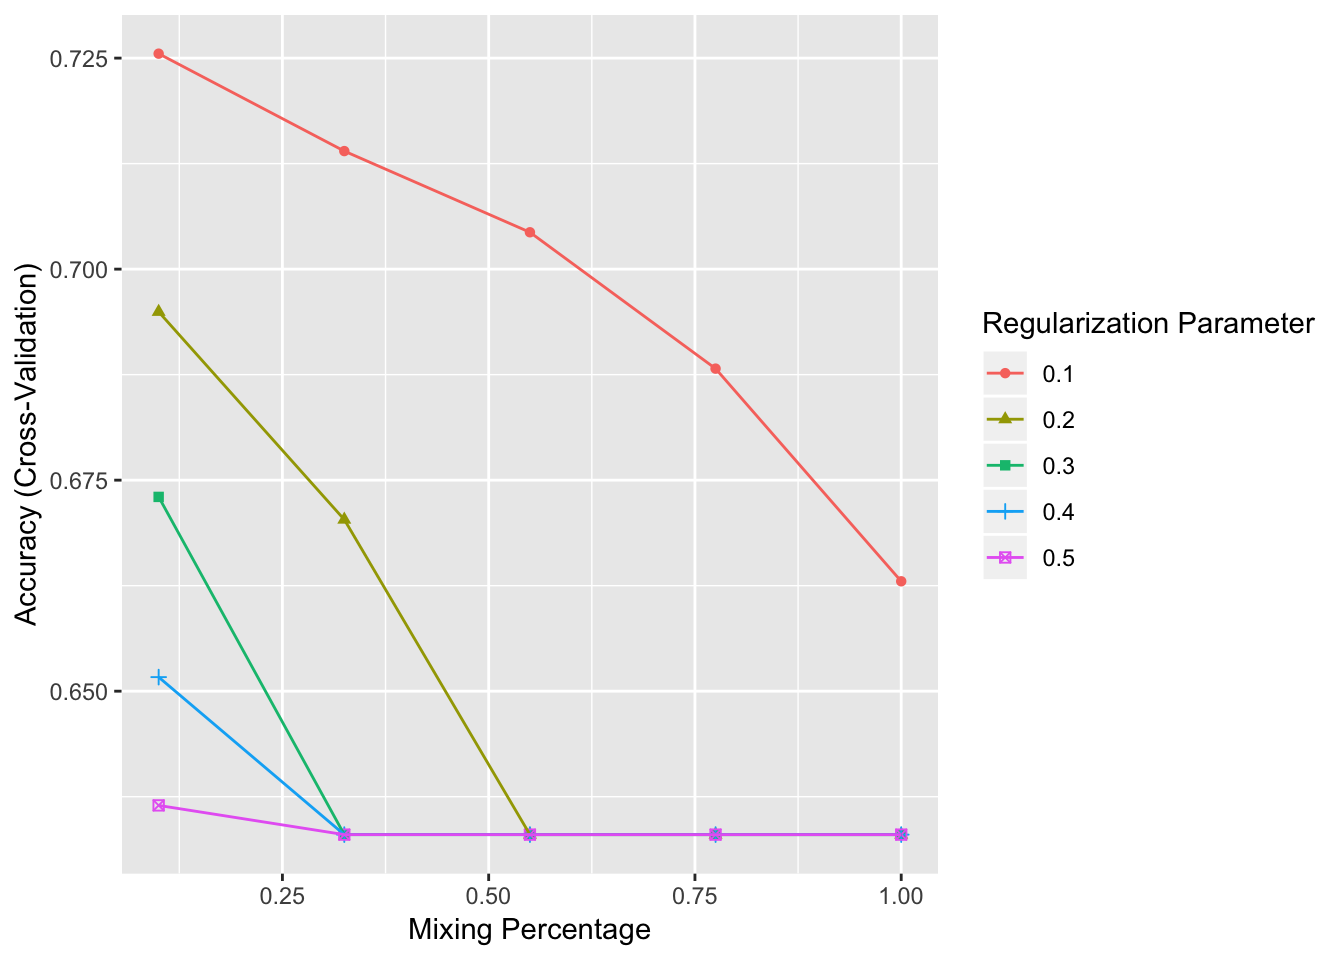
\includegraphics{Machine-Learning-MTeam_files/figure-latex/unnamed-chunk-5-1.pdf}

\begin{Shaded}
\begin{Highlighting}[]
\CommentTok{# cross validation 10}
\NormalTok{cv_opts =}\StringTok{ }\KeywordTok{trainControl}\NormalTok{(}\DataTypeTok{method=}\StringTok{'cv'}\NormalTok{, }\DataTypeTok{number=}\DecValTok{10}\NormalTok{) }\CommentTok{#定義模型訓練參數,劃分十組交叉驗證(使用repeatedcv可重複劃分)}

\NormalTok{regreg_opts =}\StringTok{ }\KeywordTok{expand.grid}\NormalTok{(}\DataTypeTok{.alpha =} \KeywordTok{seq}\NormalTok{(.}\DecValTok{1}\NormalTok{, }\DecValTok{1}\NormalTok{, }\DataTypeTok{length =} \DecValTok{5}\NormalTok{),}
                          \DataTypeTok{.lambda =} \KeywordTok{seq}\NormalTok{(.}\DecValTok{1}\NormalTok{, }\FloatTok{.5}\NormalTok{, }\DataTypeTok{length =} \DecValTok{5}\NormalTok{)) }\CommentTok{#25種組合(決定lamda重要度?)}


\NormalTok{results_regreg =}\StringTok{ }\KeywordTok{train}\NormalTok{(quality}\OperatorTok{~}\NormalTok{., }
                        \DataTypeTok{data=}\NormalTok{wine_train,}
                        \DataTypeTok{method =} \StringTok{"glmnet"}\NormalTok{, }
                        \DataTypeTok{trControl =}\NormalTok{ cv_opts, }
                        \DataTypeTok{preProcess =} \KeywordTok{c}\NormalTok{(}\StringTok{"center"}\NormalTok{, }\StringTok{"scale"}\NormalTok{), }\CommentTok{#指定數據標準化,"center"和"scale"。其中center表示預測變量減去均值}
                        \DataTypeTok{tuneGrid =}\NormalTok{ regreg_opts)}

\NormalTok{results_regreg }\CommentTok{#kappa是一統計量指標衡量預測值與實質的差距}
\end{Highlighting}
\end{Shaded}

\begin{verbatim}
## glmnet 
## 
## 5199 samples
##   10 predictor
##    2 classes: 'bad', 'good' 
## 
## Pre-processing: centered (10), scaled (10) 
## Resampling: Cross-Validated (10 fold) 
## Summary of sample sizes: 4679, 4680, 4679, 4679, 4679, 4679, ... 
## Resampling results across tuning parameters:
## 
##   alpha  lambda  Accuracy   Kappa     
##   0.100  0.1     0.7255274  0.35008588
##   0.100  0.2     0.6949431  0.24105753
##   0.100  0.3     0.6730163  0.15106604
##   0.100  0.4     0.6516660  0.07063484
##   0.100  0.5     0.6364689  0.01492729
##   0.325  0.1     0.7139856  0.31350196
##   0.325  0.2     0.6703273  0.13726298
##   0.325  0.3     0.6330066  0.00000000
##   0.325  0.4     0.6330066  0.00000000
##   0.325  0.5     0.6330066  0.00000000
##   0.550  0.1     0.7043676  0.27703468
##   0.550  0.2     0.6330066  0.00000000
##   0.550  0.3     0.6330066  0.00000000
##   0.550  0.4     0.6330066  0.00000000
##   0.550  0.5     0.6330066  0.00000000
##   0.775  0.1     0.6882142  0.21713151
##   0.775  0.2     0.6330066  0.00000000
##   0.775  0.3     0.6330066  0.00000000
##   0.775  0.4     0.6330066  0.00000000
##   0.775  0.5     0.6330066  0.00000000
##   1.000  0.1     0.6630178  0.11541687
##   1.000  0.2     0.6330066  0.00000000
##   1.000  0.3     0.6330066  0.00000000
##   1.000  0.4     0.6330066  0.00000000
##   1.000  0.5     0.6330066  0.00000000
## 
## Accuracy was used to select the optimal model using the largest value.
## The final values used for the model were alpha = 0.1 and lambda = 0.1.
\end{verbatim}

\begin{Shaded}
\begin{Highlighting}[]
\KeywordTok{ggplot}\NormalTok{(results_regreg)}
\end{Highlighting}
\end{Shaded}

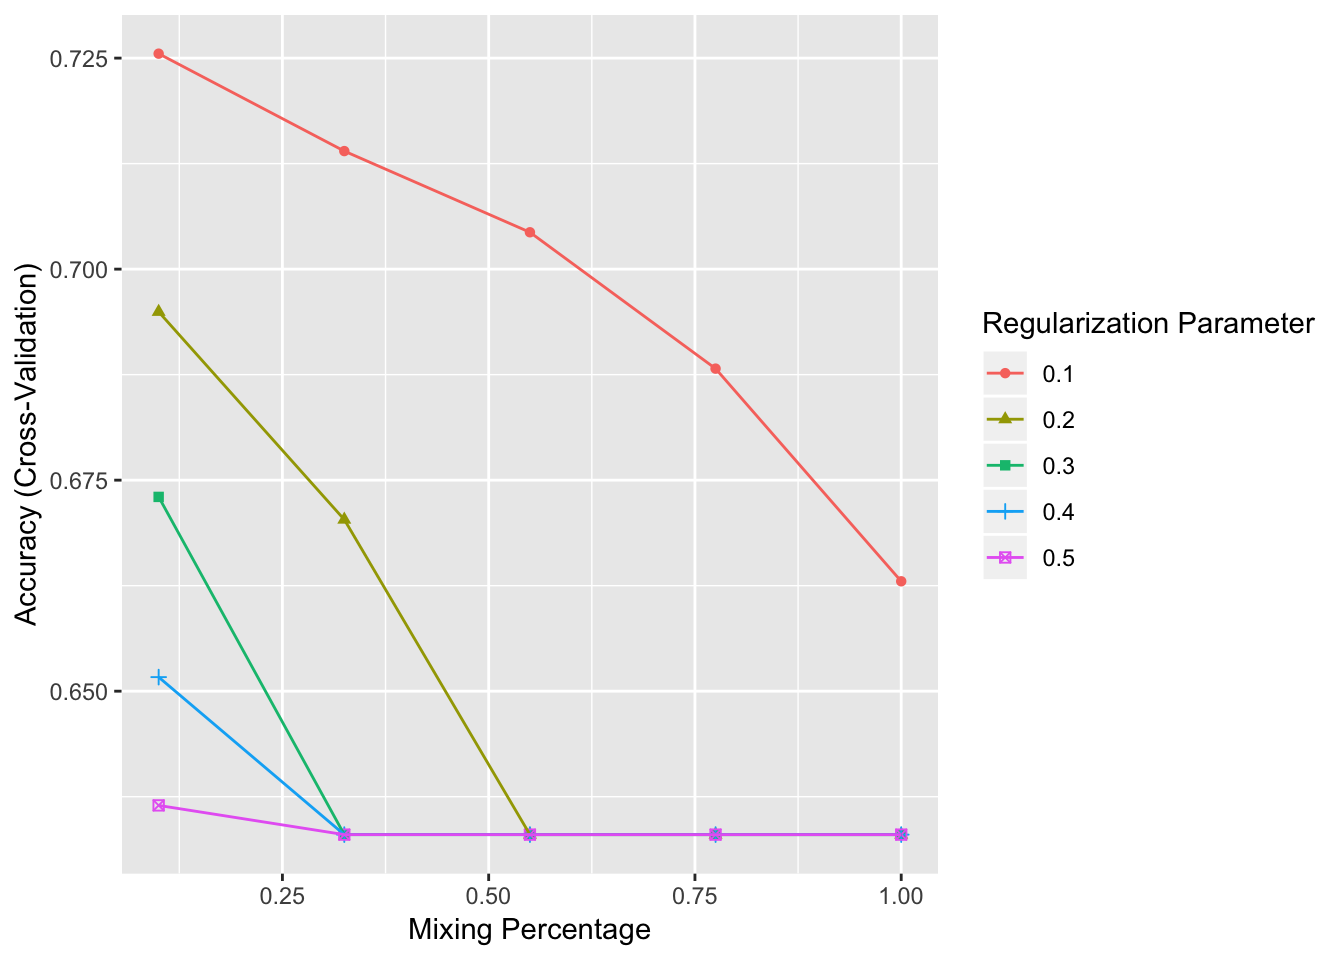
\includegraphics{Machine-Learning-MTeam_files/figure-latex/unnamed-chunk-6-1.pdf}
alpha=mixing percentage
lambda=regularization parameter

\begin{Shaded}
\begin{Highlighting}[]
\NormalTok{preds_regreg =}\StringTok{ }\KeywordTok{predict}\NormalTok{(results_regreg, wine_test)}
\NormalTok{good_observed =}\StringTok{ }\NormalTok{wine_test}\OperatorTok{$}\NormalTok{quality}
\KeywordTok{confusionMatrix}\NormalTok{(preds_regreg, good_observed, }\DataTypeTok{positive=}\StringTok{'good'}\NormalTok{) }
\end{Highlighting}
\end{Shaded}

\begin{verbatim}
## Confusion Matrix and Statistics
## 
##           Reference
## Prediction bad good
##       bad  197   76
##       good 279  746
##                                           
##                Accuracy : 0.7265          
##                  95% CI : (0.7014, 0.7506)
##     No Information Rate : 0.6333          
##     P-Value [Acc > NIR] : 6.665e-13       
##                                           
##                   Kappa : 0.3531          
##  Mcnemar's Test P-Value : < 2.2e-16       
##                                           
##             Sensitivity : 0.9075          
##             Specificity : 0.4139          
##          Pos Pred Value : 0.7278          
##          Neg Pred Value : 0.7216          
##              Prevalence : 0.6333          
##          Detection Rate : 0.5747          
##    Detection Prevalence : 0.7897          
##       Balanced Accuracy : 0.6607          
##                                           
##        'Positive' Class : good            
## 
\end{verbatim}

The lower bound (and p-value) suggests we are statistically predicting better than the No Information Rate (i.e., just guessing the more prevalent `Bad' category) -\textgreater{} 猜好的比猜壞的還強

\begin{Shaded}
\begin{Highlighting}[]
\KeywordTok{confusionMatrix}\NormalTok{(preds_regreg, good_observed, }\DataTypeTok{positive=}\StringTok{'good'}\NormalTok{, }\DataTypeTok{mode=}\StringTok{'prec_recall'}\NormalTok{)}
\end{Highlighting}
\end{Shaded}

\begin{verbatim}
## Confusion Matrix and Statistics
## 
##           Reference
## Prediction bad good
##       bad  197   76
##       good 279  746
##                                           
##                Accuracy : 0.7265          
##                  95% CI : (0.7014, 0.7506)
##     No Information Rate : 0.6333          
##     P-Value [Acc > NIR] : 6.665e-13       
##                                           
##                   Kappa : 0.3531          
##  Mcnemar's Test P-Value : < 2.2e-16       
##                                           
##               Precision : 0.7278          
##                  Recall : 0.9075          
##                      F1 : 0.8078          
##              Prevalence : 0.6333          
##          Detection Rate : 0.5747          
##    Detection Prevalence : 0.7897          
##       Balanced Accuracy : 0.6607          
##                                           
##        'Positive' Class : good            
## 
\end{verbatim}

\hypertarget{k-nearest-neighbors}{%
\chapter{k-nearest Neighbors}\label{k-nearest-neighbors}}

\begin{Shaded}
\begin{Highlighting}[]
\NormalTok{knn_opts =}\StringTok{ }\KeywordTok{data.frame}\NormalTok{(}\DataTypeTok{k=}\KeywordTok{c}\NormalTok{(}\KeywordTok{seq}\NormalTok{(}\DecValTok{3}\NormalTok{, }\DecValTok{11}\NormalTok{, }\DecValTok{2}\NormalTok{), }\DecValTok{25}\NormalTok{, }\DecValTok{51}\NormalTok{, }\DecValTok{101}\NormalTok{))}
\NormalTok{knn_opts}
\end{Highlighting}
\end{Shaded}

\begin{verbatim}
##     k
## 1   3
## 2   5
## 3   7
## 4   9
## 5  11
## 6  25
## 7  51
## 8 101
\end{verbatim}

\begin{Shaded}
\begin{Highlighting}[]
\NormalTok{results_knn =}\StringTok{ }\KeywordTok{train}\NormalTok{(quality}\OperatorTok{~}\NormalTok{., }
                    \DataTypeTok{data=}\NormalTok{wine_train, }
                    \DataTypeTok{method=}\StringTok{'knn'}\NormalTok{,}
                    \DataTypeTok{preProcess=}\KeywordTok{c}\NormalTok{(}\StringTok{'center'}\NormalTok{, }\StringTok{'scale'}\NormalTok{), }
                    \DataTypeTok{trControl=}\NormalTok{cv_opts,}
                    \DataTypeTok{tuneGrid =}\NormalTok{ knn_opts)}

\NormalTok{results_knn}
\end{Highlighting}
\end{Shaded}

\begin{verbatim}
## k-Nearest Neighbors 
## 
## 5199 samples
##   10 predictor
##    2 classes: 'bad', 'good' 
## 
## Pre-processing: centered (10), scaled (10) 
## Resampling: Cross-Validated (10 fold) 
## Summary of sample sizes: 4679, 4679, 4679, 4680, 4679, 4679, ... 
## Resampling results across tuning parameters:
## 
##   k    Accuracy   Kappa    
##     3  0.7670720  0.4901107
##     5  0.7661112  0.4848680
##     7  0.7620724  0.4740174
##     9  0.7601512  0.4700814
##    11  0.7609215  0.4691504
##    25  0.7493794  0.4373009
##    51  0.7470705  0.4273110
##   101  0.7401438  0.4042036
## 
## Accuracy was used to select the optimal model using the largest value.
## The final value used for the model was k = 3.
\end{verbatim}

\begin{Shaded}
\begin{Highlighting}[]
\NormalTok{preds_knn =}\StringTok{ }\KeywordTok{predict}\NormalTok{(results_knn, wine_test)}
\KeywordTok{confusionMatrix}\NormalTok{(preds_knn, good_observed, }\DataTypeTok{positive=}\StringTok{'good'}\NormalTok{)}
\end{Highlighting}
\end{Shaded}

\begin{verbatim}
## Confusion Matrix and Statistics
## 
##           Reference
## Prediction bad good
##       bad  296  147
##       good 180  675
##                                           
##                Accuracy : 0.7481          
##                  95% CI : (0.7235, 0.7715)
##     No Information Rate : 0.6333          
##     P-Value [Acc > NIR] : < 2e-16         
##                                           
##                   Kappa : 0.4496          
##  Mcnemar's Test P-Value : 0.07679         
##                                           
##             Sensitivity : 0.8212          
##             Specificity : 0.6218          
##          Pos Pred Value : 0.7895          
##          Neg Pred Value : 0.6682          
##              Prevalence : 0.6333          
##          Detection Rate : 0.5200          
##    Detection Prevalence : 0.6587          
##       Balanced Accuracy : 0.7215          
##                                           
##        'Positive' Class : good            
## 
\end{verbatim}

\#Neutral Network

\section{機器學習步驟}

\subsection{流程圖}

\hypertarget{cpu}{%
\subsection{CPU平行運算}\label{cpu}}

開始

\begin{Shaded}
\begin{Highlighting}[]
\KeywordTok{library}\NormalTok{(doParallel)}
\NormalTok{cl =}\StringTok{ }\KeywordTok{makeCluster}\NormalTok{(}\DecValTok{2}\NormalTok{)}
\KeywordTok{registerDoParallel}\NormalTok{(cl)}
\end{Highlighting}
\end{Shaded}

結束

\begin{Shaded}
\begin{Highlighting}[]
\KeywordTok{stopCluster}\NormalTok{(cl)}
\end{Highlighting}
\end{Shaded}

\subsection{切割資料}

\begin{Shaded}
\begin{Highlighting}[]
\KeywordTok{library}\NormalTok{(gplots)}
\KeywordTok{library}\NormalTok{(caret)}
\KeywordTok{library}\NormalTok{(tidyverse)}
\NormalTok{wine <-}\StringTok{ }\KeywordTok{read.csv}\NormalTok{(}\StringTok{'~/Dropbox/M-team/ML/wine.csv'}\NormalTok{)}
\KeywordTok{set.seed}\NormalTok{(}\DecValTok{1234}\NormalTok{) }\CommentTok{# so that the indices will be the same when re-run}
\NormalTok{trainIndices =}\StringTok{ }\KeywordTok{createDataPartition}\NormalTok{(wine}\OperatorTok{$}\NormalTok{quality, }\DataTypeTok{p=}\NormalTok{.}\DecValTok{8}\NormalTok{, }\DataTypeTok{list=}\NormalTok{F)}

\NormalTok{wine_train =}\StringTok{ }\NormalTok{wine }\OperatorTok\StringTok{ }
\StringTok{  }\KeywordTok{select}\NormalTok{(}\OperatorTok{-}\NormalTok{X,}\OperatorTok{-}\NormalTok{free.sulfur.dioxide, }\OperatorTok{-}\NormalTok{density, }\OperatorTok{-}\NormalTok{color, }\OperatorTok{-}\NormalTok{white) }\OperatorTok\StringTok{ }
\StringTok{  }\KeywordTok{slice}\NormalTok{(trainIndices)}

\NormalTok{wine_test =}\StringTok{ }\NormalTok{wine }\OperatorTok\StringTok{ }
\StringTok{  }\KeywordTok{select}\NormalTok{(}\OperatorTok{-}\NormalTok{X,}\OperatorTok{-}\NormalTok{free.sulfur.dioxide, }\OperatorTok{-}\NormalTok{density,  }\OperatorTok{-}\NormalTok{color, }\OperatorTok{-}\NormalTok{white) }\OperatorTok\StringTok{ }
\StringTok{  }\KeywordTok{slice}\NormalTok{(}\OperatorTok{-}\NormalTok{trainIndices)}

\NormalTok{wine_trainplot =}\StringTok{ }\KeywordTok{select}\NormalTok{(wine_train, }\OperatorTok{-}\NormalTok{quality) }\OperatorTok\StringTok{ }
\StringTok{  }\KeywordTok{preProcess}\NormalTok{(}\DataTypeTok{method=}\StringTok{'range'}\NormalTok{) }\OperatorTok\StringTok{ }
\StringTok{  }\KeywordTok{predict}\NormalTok{(}\DataTypeTok{newdata=} \KeywordTok{select}\NormalTok{(wine_train, }\OperatorTok{-}\NormalTok{quality))}

\NormalTok{good_observed =}\StringTok{ }\NormalTok{wine_test}\OperatorTok{$}\NormalTok{quality}
\end{Highlighting}
\end{Shaded}

\hypertarget{nnet}{%
\section{類神經網絡(NNet):}\label{nnet}}

參考資料:

\begin{itemize}
\item
  \url{https://topepo.github.io/caret/train-models-by-tag.html}
\item
  所以的模型都先看一下train-model bt tag,來看一下基本設定,以及模型特有的東西。
\end{itemize}

\hypertarget{how-the-model-is-evaluated}{%
\subsection{1. How the model is evaluated}\label{how-the-model-is-evaluated}}

Here we choose: \textbf{k-fold Cross-validation}

參考資料:\url{https://hyp.is/lc7vUNc6EeixLm87hkeo7A/m-clark.github.io/introduction-to-machine-learning/concepts.html}

10-fold CV here

\begin{Shaded}
\begin{Highlighting}[]
\NormalTok{cv_opts =}\StringTok{ }\KeywordTok{trainControl}\NormalTok{(}\DataTypeTok{method=}\StringTok{'cv'}\NormalTok{, }\DataTypeTok{number=}\DecValTok{10}\NormalTok{) }\CommentTok{# cross-validation }
\end{Highlighting}
\end{Shaded}

\hypertarget{pre-processing-setup}{%
\subsection{2. Pre-processing setup}\label{pre-processing-setup}}

\hypertarget{what-kind-of-data-transformation-is-needed-for-the-algorithm}{%
\subsubsection{2.1 What kind of data transformation is needed for the algorithm?}\label{what-kind-of-data-transformation-is-needed-for-the-algorithm}}

NNL: data requires rescaling

method = ``center'' subtracts the mean (\(mean(x)\)) of the predictor's data (again from the data in x) from the predictor values while method = ``scale'' divides by the standard deviation (\(sd(x)\)).

\[\hat{x}_i=\frac{x_i-mean(x)}{sd(x)}\]

tuneLength=5 表示 size,decay 是個5x5的grid空間。

\begin{Shaded}
\begin{Highlighting}[]
\NormalTok{results_nnet =}\StringTok{ }\KeywordTok{train}\NormalTok{(quality}\OperatorTok{~}\NormalTok{., }
                     \DataTypeTok{data=}\NormalTok{wine_train, }
                     \DataTypeTok{method=}\StringTok{'avNNet'}\NormalTok{,}
                     \DataTypeTok{trControl=}\NormalTok{cv_opts,}
                     \DataTypeTok{tuneLength=}\DecValTok{5}\NormalTok{,}
                     \DataTypeTok{preProcess=}\KeywordTok{c}\NormalTok{(}\StringTok{'center'}\NormalTok{, }\StringTok{'scale'}\NormalTok{),}
                     \DataTypeTok{trace=}\NormalTok{F, }
                     \DataTypeTok{maxit=}\DecValTok{10}\NormalTok{)}
\NormalTok{results_nnet}
\KeywordTok{ggplot}\NormalTok{(results_nnet)}
\KeywordTok{ggplot}\NormalTok{(results_nnet) }\OperatorTok{+}
\StringTok{  }\KeywordTok{labs}\NormalTok{(}\DataTypeTok{x=}\StringTok{'Number of Hidden Units'}\NormalTok{) }\OperatorTok{+}
\StringTok{  }\KeywordTok{scale_x_continuous}\NormalTok{(}\DataTypeTok{breaks =} \KeywordTok{c}\NormalTok{(}\DecValTok{1}\NormalTok{,}\DecValTok{3}\NormalTok{,}\DecValTok{5}\NormalTok{,}\DecValTok{7}\NormalTok{,}\DecValTok{9}\NormalTok{))}
\end{Highlighting}
\end{Shaded}

\begin{Shaded}
\begin{Highlighting}[]
\NormalTok{preds_nnet =}\StringTok{ }\KeywordTok{predict}\NormalTok{(results_nnet, wine_test)}
\KeywordTok{confusionMatrix}\NormalTok{(preds_nnet, good_observed, }\DataTypeTok{positive=}\StringTok{'good'}\NormalTok{)}


\CommentTok{#results_nnet1 = train(quality~., }
                    \CommentTok{# data=wine_train, }
                     \CommentTok{#method='mlpWeightDecayML',}
                     \CommentTok{#trControl=cv_opts,}
                     \CommentTok{#preProcess=c('center', 'scale'),}
                     \CommentTok{#trace=F, }
                     \CommentTok{#maxit=10)}
\CommentTok{#results_nnet1}
\end{Highlighting}
\end{Shaded}

不一定要用tuneLength由電腦選grid{[}值{]},也可改成如下的手動設定:

\begin{verbatim}
regreg_opts = expand.grid(size = seq(.1, 1, length = 5),
                          decay = seq(.1, .5, length = 5)) 
results_regreg = train( ...
                        tuneGrid = regreg_opts)
\end{verbatim}

\#Neutral Network2

\hypertarget{-1}{%
\section{機器學習步驟}\label{-1}}

\hypertarget{-1}{%
\subsection{流程圖}\label{-1}}

\hypertarget{r}{%
\subsection{1.啟用r平行運算}\label{r}}

\hypertarget{cpu-1}{%
\subsubsection{CPU平行運算}\label{cpu-1}}

\begin{Shaded}
\begin{Highlighting}[]
\KeywordTok{library}\NormalTok{(doParallel)}
\NormalTok{cl =}\StringTok{ }\KeywordTok{makeCluster}\NormalTok{(}\DecValTok{2}\NormalTok{)}
\KeywordTok{registerDoParallel}\NormalTok{(cl)}
\CommentTok{#stopCluster(cl)關閉}
\end{Highlighting}
\end{Shaded}

\subsection{2.資料處理}

\hypertarget{-1}{%
\subsubsection{切割資料}\label{-1}}

\begin{Shaded}
\begin{Highlighting}[]
\KeywordTok{library}\NormalTok{(gplots)}
\KeywordTok{library}\NormalTok{(caret)}
\KeywordTok{library}\NormalTok{(tidyverse)}
\NormalTok{wine <-}\StringTok{ }\KeywordTok{read.csv}\NormalTok{(}\StringTok{'~/Dropbox/M-team/ML/wine.csv'}\NormalTok{)}
\NormalTok{wine}\OperatorTok{$}\NormalTok{quality=}\KeywordTok{factor}\NormalTok{(wine}\OperatorTok{$}\NormalTok{quality)}
\KeywordTok{set.seed}\NormalTok{(}\DecValTok{1234}\NormalTok{) }\CommentTok{# so that the indices will be the same when re-run}
\NormalTok{trainIndices =}\StringTok{ }\KeywordTok{createDataPartition}\NormalTok{(wine}\OperatorTok{$}\NormalTok{quality, }\DataTypeTok{p=}\NormalTok{.}\DecValTok{8}\NormalTok{, }\DataTypeTok{list=}\NormalTok{F)}

\NormalTok{wine_train =}\StringTok{ }\NormalTok{wine }\OperatorTok\StringTok{ }
\StringTok{  }\KeywordTok{select}\NormalTok{(}\OperatorTok{-}\NormalTok{X,}\OperatorTok{-}\NormalTok{free.sulfur.dioxide, }\OperatorTok{-}\NormalTok{density, }\OperatorTok{-}\NormalTok{color, }\OperatorTok{-}\NormalTok{white) }\OperatorTok\StringTok{ }
\StringTok{  }\KeywordTok{slice}\NormalTok{(trainIndices)}

\NormalTok{wine_test =}\StringTok{ }\NormalTok{wine }\OperatorTok\StringTok{ }
\StringTok{  }\KeywordTok{select}\NormalTok{(}\OperatorTok{-}\NormalTok{X,}\OperatorTok{-}\NormalTok{free.sulfur.dioxide, }\OperatorTok{-}\NormalTok{density,  }\OperatorTok{-}\NormalTok{color, }\OperatorTok{-}\NormalTok{white) }\OperatorTok\StringTok{ }
\StringTok{  }\KeywordTok{slice}\NormalTok{(}\OperatorTok{-}\NormalTok{trainIndices)}

\NormalTok{wine_trainplot =}\StringTok{ }\KeywordTok{select}\NormalTok{(wine_train, }\OperatorTok{-}\NormalTok{quality) }\OperatorTok\StringTok{ }
\StringTok{  }\KeywordTok{preProcess}\NormalTok{(}\DataTypeTok{method=}\StringTok{'range'}\NormalTok{) }\OperatorTok\StringTok{ }
\StringTok{  }\KeywordTok{predict}\NormalTok{(}\DataTypeTok{newdata=} \KeywordTok{select}\NormalTok{(wine_train, }\OperatorTok{-}\NormalTok{quality))}

\NormalTok{good_observed =}\StringTok{ }\NormalTok{wine_test}\OperatorTok{$}\NormalTok{quality}
\end{Highlighting}
\end{Shaded}

\hypertarget{nnet-1}{%
\section{類神經網絡(NNet):}\label{nnet-1}}

參考資料:

\begin{itemize}
\item
  \url{https://topepo.github.io/caret/train-models-by-tag.html}
\item
  所以的模型都先看一下train-model bt tag,來看一下基本設定,以及模型特有的東西。
\end{itemize}

\hypertarget{how-the-model-is-evaluated-1}{%
\subsection{1. How the model is evaluated}\label{how-the-model-is-evaluated-1}}

Here we choose: \textbf{k-fold Cross-validation}

參考資料:\url{https://hyp.is/lc7vUNc6EeixLm87hkeo7A/m-clark.github.io/introduction-to-machine-learning/concepts.html}

10-fold CV here

\begin{Shaded}
\begin{Highlighting}[]
\NormalTok{cv_opts =}\StringTok{ }\KeywordTok{trainControl}\NormalTok{(}\DataTypeTok{method=}\StringTok{'cv'}\NormalTok{, }\DataTypeTok{number=}\DecValTok{10}\NormalTok{) }\CommentTok{# cross-validation }
\end{Highlighting}
\end{Shaded}

\hypertarget{pre-processing-setup-1}{%
\subsection{2. Pre-processing setup}\label{pre-processing-setup-1}}

\hypertarget{what-kind-of-data-transformation-is-needed-for-the-algorithm-1}{%
\subsubsection{2.1 What kind of data transformation is needed for the algorithm?}\label{what-kind-of-data-transformation-is-needed-for-the-algorithm-1}}

NNL: data requires rescaling

method = ``center'' subtracts the mean (\(mean(x)\)) of the predictor's data (again from the data in x) from the predictor values while method = ``scale'' divides by the standard deviation (\(sd(x)\)).

\[\hat{x}_i=\frac{x_i-mean(x)}{sd(x)}\]

\hypertarget{tuning-parameter-set-setup}{%
\subsection{3. (Tuning) parameter set setup}\label{tuning-parameter-set-setup}}

\hypertarget{what-are-the-tuning-parameters}{%
\subsubsection{3.1 What are the tuning parameters}\label{what-are-the-tuning-parameters}}

size: Number of hidden units

decay: 如下式數值分析的\(\eta\)

\[\theta_{i+1}=\theta_{i}-\eta\frac{\delta\ Objectivefun(\theta_i)}{\delta \theta}\]

tuneLength=5 表示 size,decay 是個5x5的grid空間。

\begin{Shaded}
\begin{Highlighting}[]
\NormalTok{results_nnet =}\StringTok{ }\KeywordTok{train}\NormalTok{(quality}\OperatorTok{~}\NormalTok{., }
                     \DataTypeTok{data=}\NormalTok{wine_train, }
                     \DataTypeTok{method=}\StringTok{'avNNet'}\NormalTok{,}
                     \DataTypeTok{trControl=}\NormalTok{cv_opts,}
                     \DataTypeTok{tuneLength=}\DecValTok{5}\NormalTok{,}
                     \DataTypeTok{preProcess=}\KeywordTok{c}\NormalTok{(}\StringTok{'center'}\NormalTok{, }\StringTok{'scale'}\NormalTok{),}
                     \DataTypeTok{trace=}\NormalTok{F, }
                     \DataTypeTok{maxit=}\DecValTok{10}\NormalTok{)}
\NormalTok{results_nnet}
\KeywordTok{ggplot}\NormalTok{(results_nnet)}
\KeywordTok{ggplot}\NormalTok{(results_nnet) }\OperatorTok{+}
\StringTok{  }\KeywordTok{labs}\NormalTok{(}\DataTypeTok{x=}\StringTok{'Number of Hidden Units'}\NormalTok{) }\OperatorTok{+}
\StringTok{  }\KeywordTok{scale_x_continuous}\NormalTok{(}\DataTypeTok{breaks =} \KeywordTok{c}\NormalTok{(}\DecValTok{1}\NormalTok{,}\DecValTok{3}\NormalTok{,}\DecValTok{5}\NormalTok{,}\DecValTok{7}\NormalTok{,}\DecValTok{9}\NormalTok{))}
\NormalTok{preds_nnet =}\StringTok{ }\KeywordTok{predict}\NormalTok{(results_nnet, wine_test)}
\KeywordTok{confusionMatrix}\NormalTok{(preds_nnet, good_observed, }\DataTypeTok{positive=}\StringTok{'good'}\NormalTok{)}


\CommentTok{#results_nnet1 = train(quality~., }
                    \CommentTok{# data=wine_train, }
                     \CommentTok{#method='mlpWeightDecayML',}
                     \CommentTok{#trControl=cv_opts,}
                     \CommentTok{#preProcess=c('center', 'scale'),}
                     \CommentTok{#trace=F, }
                     \CommentTok{#maxit=10)}
\CommentTok{#results_nnet1}
\end{Highlighting}
\end{Shaded}

不一定要用tuneLength由電腦選grid{[}值{]},也可改成如下的手動設定:

\begin{verbatim}
regreg_opts = expand.grid(size = seq(.1, 1, length = 5),
                          decay = seq(.1, .5, length = 5)) 
results_regreg = train( ...
                        tuneGrid = regreg_opts)
\end{verbatim}

\#Trees and Forests

\section{隨機森林}

參考資料:\url{https://topepo.github.io/caret/train-models-by-tag.html\#Random_Forest}

\subsection{1. 概念}

\hypertarget{decision-tree-classifier}{%
\subsubsection{1.1 Decision tree classifier}\label{decision-tree-classifier}}

\href{https://medium.com/machine-learning-101/chapter-3-decision-trees-theory-e7398adac567}{Basic concept}: 非常清楚的說明

\href{https://scikit-learn.org/stable/modules/generated/sklearn.tree.DecisionTreeClassifier.html\#sklearn.tree.DecisionTreeClassifier}{scikit code documentation}

\hypertarget{random-forest-classifier}{%
\subsubsection{1.2 Random forest classifier}\label{random-forest-classifier}}

給定一組training data,演算法會決定那一棵樹最適合它(?)。Random forest透過Boostrapping產生如1000個training data,每個用來找一棵最適合它的樹,最後以這1000顆樹來衡量它對真正test data的預測(採多數決)。

\hypertarget{cross-validation-pre-processing}{%
\subsection{2. Cross-Validation \& Pre processing}\label{cross-validation-pre-processing}}

同前

\hypertarget{tuning-parameters}{%
\subsection{3. Tuning parameters}\label{tuning-parameters}}

mtry: 隨機選出來用來架構樹之節點的特徵變數個數

\begin{quote}
In addition, when splitting a node during the construction of the tree, the split that is chosen (即用什麼特徵變數來進一步分類) is no longer the best split among all features. Instead, the split that is picked is the best split among a random subset of the features. \ldots{}\href{https://scikit-learn.org/stable/modules/ensemble.html\#forest}{scikit code documentation}
\end{quote}

ntree: 透過Boostrapping來產生「找樹用的」training data(一組樣本找一顆)。

\begin{Shaded}
\begin{Highlighting}[]
\NormalTok{rf_opts =}\StringTok{ }\KeywordTok{data.frame}\NormalTok{(}\DataTypeTok{mtry=}\KeywordTok{c}\NormalTok{(}\DecValTok{2}\OperatorTok{:}\DecValTok{6}\NormalTok{))}
\NormalTok{results_rf =}\StringTok{ }\KeywordTok{train}\NormalTok{(quality}\OperatorTok{~}\NormalTok{., }
                   \DataTypeTok{data =}\NormalTok{ wine_train,}
                   \DataTypeTok{method =} \StringTok{'rf'}\NormalTok{,}
                   \DataTypeTok{preProcess =} \KeywordTok{c}\NormalTok{(}\StringTok{'center'}\NormalTok{, }\StringTok{'scale'}\NormalTok{),}
                   \DataTypeTok{trControl =}\NormalTok{ cv_opts,}
                   \DataTypeTok{tuneGrid =}\NormalTok{ rf_opts,}
                   \DataTypeTok{localImp =}\NormalTok{ T,}
                   \DataTypeTok{ntree=}\DecValTok{100}\NormalTok{)}
\NormalTok{results_rf}
\NormalTok{preds_rf =}\StringTok{ }\KeywordTok{predict}\NormalTok{(results_rf, wine_test)}
\NormalTok{preds_rf}
\KeywordTok{confusionMatrix}\NormalTok{(preds_rf, good_observed, }\DataTypeTok{positive=}\StringTok{'good'}\NormalTok{)}
\end{Highlighting}
\end{Shaded}

\subsection{4. 各別變數的重要性}

\textbf{參考資料}: \url{https://cran.rstudio.com/web/packages/randomForestExplainer/vignettes/randomForestExplainer.html}

\subsubsection{4.1 基本概念}

\begin{Shaded}
\begin{Highlighting}[]
\KeywordTok{varImp}\NormalTok{(results_rf)}
\end{Highlighting}
\end{Shaded}

\textless{}\textless{}\textless{}\textless{}\textless{}\textless{}\textless{} HEAD:機器學習-類神經網絡,隨機森林.Rmd
\textgreater{} 兩個問題:

\begin{enumerate}
\def\labelenumi{\arabic{enumi}.}
\item
  minimum depth 出現兩次,要怎麼算是他是第1/2/1.5次數
\item ~
  \hypertarget{interactionunconditional-term}{%
  \chapter{interaction裡面unconditional term是什麼意思?}\label{interactionunconditional-term}}
\end{enumerate}

\subsubsection{4.2 重要性與樹的結構關連}

\begin{quote}
\begin{quote}
\begin{quote}
\begin{quote}
\begin{quote}
\begin{quote}
\begin{quote}
Martin:機器學習-類神經網絡,隨機森林-Martin.Rmd
\end{quote}
\end{quote}
\end{quote}
\end{quote}
\end{quote}
\end{quote}
\end{quote}

\begin{Shaded}
\begin{Highlighting}[]
\KeywordTok{library}\NormalTok{(randomForestExplainer)}
\KeywordTok{plot_min_depth_distribution}\NormalTok{(results_rf}\OperatorTok{$}\NormalTok{finalModel)}
\end{Highlighting}
\end{Shaded}

\subsubsection{4.3 交叉項的重要性}

? 用來更加突顯某一變數帶給其他變數的重要性?

\begin{Shaded}
\begin{Highlighting}[]
\KeywordTok{plot_min_depth_interactions}\NormalTok{(results_rf}\OperatorTok{$}\NormalTok{finalModel, }\DataTypeTok{k=}\DecValTok{7}\NormalTok{)}

\NormalTok{multi_imps =}\StringTok{ }\KeywordTok{measure_importance}\NormalTok{(results_rf}\OperatorTok{$}\NormalTok{finalModel)}
\KeywordTok{plot_importance_ggpairs}\NormalTok{(multi_imps)}
\end{Highlighting}
\end{Shaded}

\begin{quote}
視覺化的圖,是預測的結果,若預測結果是0.8,表示Random Forest若有1000顆樹,有800顆樹認為他是好的,可是若看到是紅色的,表示本質上他是壞的,這樣就是不成功的預測。很順利的Random Forest就會把它分個很開,很成功。
\end{quote}

\begin{Shaded}
\begin{Highlighting}[]
\CommentTok{# https://arxiv.org/pdf/1501.07196}
\CommentTok{# tibble causes problem so convert wine_train to standard df.}
\KeywordTok{library}\NormalTok{(ggRandomForests)}
\NormalTok{rf2 =}\StringTok{ }\KeywordTok{rfsrc}\NormalTok{(}\DataTypeTok{formula =}\NormalTok{ quality }\OperatorTok{~}\NormalTok{., }
            \DataTypeTok{data =} \KeywordTok{data.frame}\NormalTok{(wine_train),}
            \DataTypeTok{mtry =}\NormalTok{ results_rf}\OperatorTok{$}\NormalTok{finalModel}\OperatorTok{$}\NormalTok{mtry)}
\NormalTok{gg_v =}\StringTok{ }\KeywordTok{gg_variable}\NormalTok{(rf2)}
\NormalTok{gg_md =}\StringTok{ }\KeywordTok{gg_minimal_depth}\NormalTok{(rf2)}

\CommentTok{# We want the top two ranked minimal depth variables only}
\NormalTok{xvar =}\StringTok{ }\NormalTok{gg_md}\OperatorTok{$}\NormalTok{topvars[}\DecValTok{1}\OperatorTok{:}\DecValTok{2}\NormalTok{]}
\KeywordTok{plot}\NormalTok{(gg_v, }\DataTypeTok{xvar=}\NormalTok{xvar, }\DataTypeTok{panel=}\OtherTok{TRUE}\NormalTok{, }\DataTypeTok{partial=}\OtherTok{TRUE}\NormalTok{, }\DataTypeTok{alpha=}\NormalTok{.}\DecValTok{1}\NormalTok{)}
\end{Highlighting}
\end{Shaded}

\textless{}\textless{}\textless{}\textless{}\textless{}\textless{}\textless{} HEAD:機器學習-類神經網絡,隨機森林.Rmd
\#\#\# LIME 用一個簡單的分類方式,去嘗試去彌補複雜模型的不易詮釋狀況。

{[}\url{https://via.hypothes.is/https://medium.com/@kstseng/lime-local-interpretable-model-agnostic-explanation-技術介紹-a67b6c34c3f8}{]}

\hypertarget{lime}{%
\section{LIME}\label{lime}}

\begin{Shaded}
\begin{Highlighting}[]
\KeywordTok{library}\NormalTok{(dplyr)}

\KeywordTok{set.seed}\NormalTok{(}\DecValTok{1234}\NormalTok{)}
\NormalTok{sample_index =}\StringTok{ }\KeywordTok{sample}\NormalTok{(}\DecValTok{1}\OperatorTok{:}\KeywordTok{nrow}\NormalTok{(wine_test), }\DecValTok{5}\NormalTok{)}
\NormalTok{sample_test =}\StringTok{ }\NormalTok{wine_test }\OperatorTok\StringTok{ }
\StringTok{  }\KeywordTok{slice}\NormalTok{(sample_index) }\OperatorTok\StringTok{ }
\StringTok{  }\KeywordTok{select}\NormalTok{(}\OperatorTok{-}\NormalTok{quality)}

\KeywordTok{library}\NormalTok{(lime)}
\NormalTok{rf_lime =}\StringTok{ }\KeywordTok{lime}\NormalTok{(wine_train, results_rf)}
\NormalTok{rf_explain =}\StringTok{ }\KeywordTok{explain}\NormalTok{(sample_test, }
\NormalTok{                     rf_lime, }
                     \DataTypeTok{n_features =} \DecValTok{3}\NormalTok{,}
                     \DataTypeTok{feature_select =} \StringTok{'highest_weights'}\NormalTok{,}
                     \DataTypeTok{labels =} \StringTok{'Good'}\NormalTok{)}
\end{Highlighting}
\end{Shaded}

=======
\#\#\# 5 LIME

每一瓶酒

\begin{enumerate}
\def\labelenumi{\arabic{enumi}.}
\tightlist
\item
  Permute the data n times to create data with similar distributional properties to the original.
\end{enumerate}

\begin{itemize}
\tightlist
\item
  創造相似的酒(特徵變化要符合原始資料特徴間的統計性質,如變異及相關程度)
\end{itemize}

\begin{enumerate}
\def\labelenumi{\arabic{enumi}.}
\setcounter{enumi}{1}
\tightlist
\item
  Get similarity scores of the permuted observations to the observations you wish to explain.
\end{enumerate}

\begin{itemize}
\tightlist
\item
  依相似度要計算與原本那瓶酒的 「相似度」,之後權重用。
\end{itemize}

\begin{enumerate}
\def\labelenumi{\arabic{enumi}.}
\setcounter{enumi}{2}
\tightlist
\item
  Make predictions with the permuted data based on the ML model.
\end{enumerate}

\begin{itemize}
\tightlist
\item
  對新樣本做ML分類。
\end{itemize}

\begin{enumerate}
\def\labelenumi{\arabic{enumi}.}
\setcounter{enumi}{3}
\tightlist
\item
  Select m features (e.g.~forward selection, lasso) best describing the complex model outcome from the permuted data.
\end{enumerate}

\begin{itemize}
\tightlist
\item
  選擇一組你想理解對ML結果影響重要的特徵。
\end{itemize}

\begin{enumerate}
\def\labelenumi{\arabic{enumi}.}
\setcounter{enumi}{4}
\tightlist
\item
  Fit a simple model, e.g.~standard regression, predicting the predictions from the ML model with the m features, where observations are weighted by similarity to the to-be-explained observations.
\end{enumerate}

\begin{itemize}
\tightlist
\item
  對摸擬樣本為如好酒的機率,對這組特徵進行加權迴歸,係數值越大的越重要。
\end{itemize}

\paragraph{5.1 圖形解釋}

\begin{quote}
\begin{quote}
\begin{quote}
\begin{quote}
\begin{quote}
\begin{quote}
\begin{quote}
Martin:機器學習-類神經網絡,隨機森林-Martin.Rmd
\end{quote}
\end{quote}
\end{quote}
\end{quote}
\end{quote}
\end{quote}
\end{quote}

\#Trees and Forests2

\hypertarget{-1}{%
\section{隨機森林}\label{-1}}

參考資料:\url{https://topepo.github.io/caret/train-models-by-tag.html\#Random_Forest}

\hypertarget{-1}{%
\subsection{1. 概念}\label{-1}}

\hypertarget{decision-tree-classifier-1}{%
\subsubsection{1.1 Decision tree classifier}\label{decision-tree-classifier-1}}

\href{https://medium.com/machine-learning-101/chapter-3-decision-trees-theory-e7398adac567}{Basic concept}: 非常清楚的說明

\href{https://scikit-learn.org/stable/modules/generated/sklearn.tree.DecisionTreeClassifier.html\#sklearn.tree.DecisionTreeClassifier}{scikit code documentation}

\hypertarget{random-forest-classifier-1}{%
\subsubsection{1.2 Random forest classifier}\label{random-forest-classifier-1}}

給定一組training data,演算法會決定那一棵樹最適合它(?)。Random forest透過Boostrapping產生如1000個training data,每個用來找一棵最適合它的樹,最後以這1000顆樹來衡量它對真正test data的預測(採多數決)。

\hypertarget{cross-validation-pre-processing-1}{%
\subsection{2. Cross-Validation \& Pre processing}\label{cross-validation-pre-processing-1}}

同前

\hypertarget{tuning-parameters-1}{%
\subsection{3. Tuning parameters}\label{tuning-parameters-1}}

mtry: 隨機選出來用來架構樹之節點的特徵變數個數

\begin{quote}
In addition, when splitting a node during the construction of the tree, the split that is chosen (即用什麼特徵變數來進一步分類) is no longer the best split among all features. Instead, the split that is picked is the best split among a random subset of the features. \ldots{}\href{https://scikit-learn.org/stable/modules/ensemble.html\#forest}{scikit code documentation}
\end{quote}

ntree: 透過Boostrapping來產生「找樹用的」training data(一組樣本找一顆)。

\begin{Shaded}
\begin{Highlighting}[]
\NormalTok{rf_opts =}\StringTok{ }\KeywordTok{data.frame}\NormalTok{(}\DataTypeTok{mtry=}\KeywordTok{c}\NormalTok{(}\DecValTok{2}\OperatorTok{:}\DecValTok{6}\NormalTok{))}
\NormalTok{results_rf =}\StringTok{ }\KeywordTok{train}\NormalTok{(quality}\OperatorTok{~}\NormalTok{., }
                   \DataTypeTok{data =}\NormalTok{ wine_train,}
                   \DataTypeTok{method =} \StringTok{'rf'}\NormalTok{,}
                   \DataTypeTok{preProcess =} \KeywordTok{c}\NormalTok{(}\StringTok{'center'}\NormalTok{, }\StringTok{'scale'}\NormalTok{),}
                   \DataTypeTok{trControl =}\NormalTok{ cv_opts,}
                   \DataTypeTok{tuneGrid =}\NormalTok{ rf_opts,}
                   \DataTypeTok{localImp =}\NormalTok{ T,}
                   \DataTypeTok{ntree=}\DecValTok{10}\NormalTok{)}
\NormalTok{results_rf}
\end{Highlighting}
\end{Shaded}

\hypertarget{make-confusionm-matrix}{%
\subsection{4. make confusionm matrix}\label{make-confusionm-matrix}}

參考資料:\url{https://hyp.is/f2kmRgEUEemKAFeGta_7RA/m-clark.github.io/introduction-to-machine-learning/opening-the-black-box.html}

\begin{Shaded}
\begin{Highlighting}[]
\NormalTok{preds_rf =}\StringTok{ }\KeywordTok{predict}\NormalTok{(results_rf, wine_test)}
\NormalTok{preds_rf}
\KeywordTok{confusionMatrix}\NormalTok{(preds_rf, good_observed, }\DataTypeTok{positive=}\StringTok{'good'}\NormalTok{)}
\end{Highlighting}
\end{Shaded}

利用confusionMatrix觀察模型衡量指標(準確率、召回率...)並依照研究問題判斷模型適不適合。

\subsection{5. 變數重要性衡量}

\textbf{參考資料}: \url{https://cran.rstudio.com/web/packages/randomForestExplainer/vignettes/randomForestExplainer.html}

\hypertarget{vimp}{%
\subsubsection{5.1 VIMP}\label{vimp}}

概念:利用特徵經過置換前與置換後的誤差影響,來衡量該特徵的重要性。

步驟:

\begin{enumerate}
\def\labelenumi{\arabic{enumi}.}
\tightlist
\item
  利用每棵樹的分類模型來預測自己的OOB樣本,並計算錯誤率。
\end{enumerate}

\begin{itemize}
\tightlist
\item
  OOB:在建構每棵樹的時候,我們對訓練集使用了不同的bootstrap sample。所以對於每棵樹而言,大约有1/3的資料點是沒有參與該棵樹的生成,他們就是該棵樹的OOB样本。
\end{itemize}

\begin{enumerate}
\def\labelenumi{\arabic{enumi}.}
\setcounter{enumi}{1}
\item
  對想了解該特徵重要性的特徵進行隨機打亂,例如:把各資料點的「酒精濃度」進行隨機打亂。
\item
  利用原隨機森林模型進行預測得到新的outcome。
\item
  計算每棵樹新的OOB樣本錯誤率。
\item
  對於每棵樹擾亂特徵前後所得到的錯誤率相減並平均。
\item
  得出因該特徵擾亂後而導致的平均誤差上升多少,越高代表該變數越重要。
\end{enumerate}

\begin{Shaded}
\begin{Highlighting}[]
\KeywordTok{varImp}\NormalTok{(results_rf)}
\end{Highlighting}
\end{Shaded}

\hypertarget{minimal-depth}{%
\subsubsection{5.2 Minimal depth}\label{minimal-depth}}

概念:每棵樹在生成每個節點時都會有一個特徵,在樹越上層(越淺)的特徵重要程度會越大,利用此特點來計算特徵的平均最小深度觀察特徵的重要性。

補充:假設森林有兩棵樹,A樹中特徵「酒精濃度」出現在第一層,B樹中「酒精濃度」出現在第二層與第四層,那麼平均最小深度為(\(\frac{7}{3}\))

\begin{Shaded}
\begin{Highlighting}[]
\KeywordTok{library}\NormalTok{(randomForestExplainer)}
\KeywordTok{plot_min_depth_distribution}\NormalTok{(results_rf}\OperatorTok{$}\NormalTok{finalModel)}
\KeywordTok{plot_min_depth_interactions}\NormalTok{(results_rf}\OperatorTok{$}\NormalTok{finalModel, }\DataTypeTok{k=}\DecValTok{7}\NormalTok{)}
\end{Highlighting}
\end{Shaded}

\hypertarget{other-measures}{%
\subsubsection{5.3 Other Measures}\label{other-measures}}

參考資料:\url{https://cran.r-project.org/web/packages/randomForestExplainer/vignettes/randomForestExplainer.html}

\begin{Shaded}
\begin{Highlighting}[]
\NormalTok{multi_imps =}\StringTok{ }\KeywordTok{measure_importance}\NormalTok{(results_rf}\OperatorTok{$}\NormalTok{finalModel)}
\KeywordTok{plot_importance_ggpairs}\NormalTok{(multi_imps)}
\end{Highlighting}
\end{Shaded}

\subsection{6. 觀察兩兩變數之關係}

參考資料:ggRandomForests \url{https://arxiv.org/pdf/1501.07196}

\begin{Shaded}
\begin{Highlighting}[]
\CommentTok{# tibble causes problem so convert wine_train to standard df.}
\KeywordTok{library}\NormalTok{(ggRandomForests)}
\NormalTok{rf2 =}\StringTok{ }\KeywordTok{rfsrc}\NormalTok{(}\DataTypeTok{formula =}\NormalTok{ quality }\OperatorTok{~}\NormalTok{., }
            \DataTypeTok{data =} \KeywordTok{data.frame}\NormalTok{(wine_train),}
            \DataTypeTok{mtry =}\NormalTok{ results_rf}\OperatorTok{$}\NormalTok{finalModel}\OperatorTok{$}\NormalTok{mtry)}
\NormalTok{gg_v =}\StringTok{ }\KeywordTok{gg_variable}\NormalTok{(rf2)}
\NormalTok{gg_md =}\StringTok{ }\KeywordTok{gg_minimal_depth}\NormalTok{(rf2)}
\NormalTok{gg_v}
\NormalTok{gg_md}
\NormalTok{xvar =}\StringTok{ }\NormalTok{gg_md}\OperatorTok{$}\NormalTok{topvars[}\DecValTok{1}\OperatorTok{:}\DecValTok{2}\NormalTok{]}\CommentTok{#表示取出前兩個最重要的變數。}
\KeywordTok{plot}\NormalTok{(gg_v, }\DataTypeTok{xvar=}\NormalTok{xvar, }\DataTypeTok{panel=}\OtherTok{TRUE}\NormalTok{, }\DataTypeTok{partial=}\OtherTok{TRUE}\NormalTok{, }\DataTypeTok{alpha=}\NormalTok{.}\DecValTok{1}\NormalTok{)}
\end{Highlighting}
\end{Shaded}

圖中縱軸為模型判定為good的機率,每一個點代表一個資料點,顏色為該資料點的真實outcome,以點(10,0.75,紅)為例;表示有一瓶酒,其酒精濃度為10且1000棵樹裡面有750棵說他是good(0.75),但它實際上是壞的(紅色)。

\hypertarget{lime-1}{%
\subsection{7. LIME}\label{lime-1}}

LIME 想要解決的問題:找到一個容易解釋的模型 g 解釋為什麼一個個體會被分類到f預測的類別;f是依據什麼特徵來分類進一步了解各特徵的重要性。

參考資料: \url{https://medium.com/@kstseng/lime-local-interpretable-model-agnostic-explanation-\%E6\%8A\%80\%E8\%A1\%93\%E4\%BB\%8B\%E7\%B4\%B9-a67b6c34c3f8}

步驟:

每一瓶酒

\begin{enumerate}
\def\labelenumi{\arabic{enumi}.}
\tightlist
\item
  Permute the data n times to create data with similar distributional properties to the original.
\end{enumerate}

\begin{itemize}
\item
  創造相似的酒(特徵變化要符合原始資料特徴間的統計性質,如變異及相關程度)。

  擾動樣本:進行有意義的擾動(改變\({x}_i\)的幾個特徵值),產生新的輸入資料\({z}_i\)。
\end{itemize}

\begin{enumerate}
\def\labelenumi{\arabic{enumi}.}
\setcounter{enumi}{1}
\tightlist
\item
  Get similarity scores of the permuted observations to the observations you wish to explain.
\end{enumerate}

\begin{itemize}
\tightlist
\item
  依相似度要計算與原本那瓶酒的 「相似度」;與原資料的距離越近者給予的係數 \(\pi_{{x}_i}\) 越大,之後權重用。
\end{itemize}

\begin{enumerate}
\def\labelenumi{\arabic{enumi}.}
\setcounter{enumi}{2}
\tightlist
\item
  Make predictions with the permuted data based on the ML model.
\end{enumerate}

\begin{itemize}
\tightlist
\item
  對新樣本(\({z}_i\))做ML分類得到新樣本得預測結果g(z)。
\end{itemize}

\begin{enumerate}
\def\labelenumi{\arabic{enumi}.}
\setcounter{enumi}{3}
\tightlist
\item
  Min loss function : \(\sum\pi_{{x}_i}(f(z)-g(z))^2+ \Omega(g)\)
\end{enumerate}

\begin{itemize}
\tightlist
\item
  f(z)為真實outcome,\(\Omega(g)\)為懲罰項目的為希望g能簡單一點,\(\pi_{{x}_i}\)為「與\({x}_i\)相似與否」的核函數。極小化loss function 找出最適的g。
\end{itemize}

\begin{enumerate}
\def\labelenumi{\arabic{enumi}.}
\setcounter{enumi}{3}
\tightlist
\item
  Select m features (e.g.~forward selection, lasso) best describing the complex model outcome from the permuted data.
\end{enumerate}

\begin{itemize}
\tightlist
\item
  選擇一組你想理解對ML結果影響重要的特徵。
\end{itemize}

\begin{enumerate}
\def\labelenumi{\arabic{enumi}.}
\setcounter{enumi}{4}
\tightlist
\item
  Fit a simple model, e.g.~standard regression, predicting the predictions from the ML model with the m features, where observations are weighted by similarity to the to-be-explained observations.
\end{enumerate}

\begin{itemize}
\tightlist
\item
  對摸擬樣本\({z}_i\)與選好的幾個特徵進行加權迴歸(model g),觀察各特徵係數值;係數值越大者越重要。
\end{itemize}

因為LIME很吃電腦資源所以下例程式碼中只隨機挑選了5個case(5個資料點)進行LIME

\begin{Shaded}
\begin{Highlighting}[]
\KeywordTok{set.seed}\NormalTok{(}\DecValTok{1234}\NormalTok{)}
\NormalTok{sample_index =}\StringTok{ }\KeywordTok{sample}\NormalTok{(}\DecValTok{1}\OperatorTok{:}\KeywordTok{nrow}\NormalTok{(wine_test), }\DecValTok{5}\NormalTok{)}\CommentTok{#隨機選取幾個case}
\NormalTok{sample_test =}\StringTok{ }\NormalTok{wine_test }\OperatorTok\StringTok{ }
\StringTok{  }\KeywordTok{slice}\NormalTok{(sample_index) }\OperatorTok\StringTok{ }
\StringTok{  }\KeywordTok{select}\NormalTok{(}\OperatorTok{-}\NormalTok{quality) }\CommentTok{#分別拿掉5個case的outcome}
\KeywordTok{library}\NormalTok{(lime)}
\NormalTok{rf_lime =}\StringTok{ }\KeywordTok{lime}\NormalTok{(wine_train, results_rf)}\CommentTok{#lime}
\NormalTok{rf_explain =}\StringTok{ }\KeywordTok{explain}\NormalTok{(sample_test, }
\NormalTok{                     rf_lime, }
                     \DataTypeTok{n_features =} \DecValTok{3}\NormalTok{,}\CommentTok{#只看三種特徵的組合}
                     \DataTypeTok{feature_select =} \StringTok{'highest_weights'}\NormalTok{,}
                     \DataTypeTok{labels =} \StringTok{'good'}\NormalTok{)}
\NormalTok{rf_explain}\CommentTok{#各case跑完lime的係數狀況}
\KeywordTok{plot_features}\NormalTok{(rf_explain)}
\KeywordTok{plot_explanations}\NormalTok{(rf_explain)}
\end{Highlighting}
\end{Shaded}

以case 1 為例:

\begin{itemize}
\tightlist
\item
  Probablity為預測good的機率
\item
  feature\_weight為-0.15表示當「0.40 \textless{} volatile.acidity」時,每增加一單位酸度y便會造成減少0.16。
\item
  \[y = \left\{\begin{array}{ll}
               bad, & \mbox{if $y<0$} \\  
               good, & \mbox{if $y>0$} \\  
              \end{array} \right.\]
\item
  Explanation為\(R^2\)
\end{itemize}

\hypertarget{svm}{%
\chapter{SVM}\label{svm}}

\hypertarget{-2}{%
\section{概念}\label{-2}}

Features: \(x_i\), Outcome: \(y_i\in {0,1}\),

\begin{itemize}
\tightlist
\item
  supporting hyperplane (SupH): any \(w,b,\delta\) that can satisfy \(w^Tx_i\geq b+\delta\) iff \(y_i>0\) and \(w^Tx_i\leq b-\delta\) iff \(y_i<0\). The equality holds for some points in each area, i.e.~at least one point \textbf{touchs} each plane. 數學上兩個supporting hyperplanes可以寫成:
\end{itemize}

\[supH_1: w^Tx=b+\delta\]
\[supH_2: w^Tx=b-\delta\]

\begin{itemize}
\tightlist
\item
  separating hypoerplane (SepH): the hyperplane that lies in the middle of the two SupHs. 數學上Separating hyperplane可以寫成:
\end{itemize}

\[w^Tx=b\]

\begin{itemize}
\tightlist
\item
  margin: 兩個supHs的距離.
\end{itemize}

目標在極大化margin,使Supporting hyperplane分割空間越清楚越好,數學上來說它等同於極小化\(\|w\|\),故可以寫成:

\[min_{\{w,b,\delta\}}\ \|w\|^2\]

受限於:

\[when\ (y_i=1,x_i),\ w^Tx_i-(b+\delta)\geq 0\]
\[when\ (y_i=-1,x_i),\ w^Tx_i-(b-\delta)\leq 0\]
他們等同於:

\[\begin{eqnarray*}
when\ y_i=1,\ (w^{T}x_{i}-(b+\delta))y_{i} & \geq & 0\\
when\ y_i=-1,\ (w^{T}x_{i}-(b-\delta))y_{i} & \geq & 0
\end{eqnarray*}
\]
也就是:
\[(w^Tx_i-b)y_i-\delta \geq 0\]

\hypertarget{algorithm-summary}{%
\subsubsection{Algorithm Summary}\label{algorithm-summary}}

\[min_{\{w,b,\delta\}}\ \frac{1}{2}\|w\|^2\]
\[s.t.\ (w^Tx_i-b)y_i-\delta\geq 0\]
If \((w^*,b^*,\delta^*)\) is a possible solution, \(\lambda (w^*,b^*,\delta^*)\) for \(\lambda>0\) will be a solution too. Therefore, we normalize \(\delta=1\).

\[min_{\{w,b,\delta\}}\ \frac{1}{2}\|w\|^2\]
\[s.t.\ (w^Tx_i-b)y_i-1\geq 0\]
Then do the Lagrange Multiplier.

\hypertarget{kernel-function}{%
\subsubsection{Kernel Function}\label{kernel-function}}

The whole discusstion above is about linear data, if not, we should mapping data to a higher dimension by Kernel Function.

\[x_i^Tx_j\rightarrow\emptyset(x_i)^T\emptyset(x_j)\]

The kernel function could be very complicated, but by inner product, it will be simple a lot.
\[K(x_i,x_j)\rightarrow\emptyset(x_i)^T\emptyset(x_j)\]
\[K(x_i,x_j)\rightarrow\exp(-\frac{\|x_i-x_j||^2}{2\sigma^2})\]

\hypertarget{the-non-separable-case}{%
\subsection{The Non-Separable case}\label{the-non-separable-case}}

In real world, it is hard to find a optimal separating hyperplane(OSH), we need to insert a error term to handle the case that support vectors overlap with SupHs.

\[w^Tx_i-b\leq-1+\xi_i\  \forall y_i=-1\]
\[w^Tx_i-b\geq+1-\xi_i\  \forall y_i=+1\]
\[\xi_i\geq0\]
and made a cost function(``c'' is the weight of cost):

\[cost = c(\sum_i\xi_i)^k\]
then

\[min\ \frac{1}{2}\|w\|^2+c(\sum_i\xi_i)^k\]
\[s.t.\ (w^Tx_i-b)y_i-1+\xi_i\geq 0\]

\hypertarget{r-code-example}{%
\section{R-code example}\label{r-code-example}}

\hypertarget{cross-validation-pre-processing-2}{%
\subsection{Cross-Validation \& Pre processing}\label{cross-validation-pre-processing-2}}

as above

\hypertarget{tuning-parameters-2}{%
\subsection{Tuning parameters}\label{tuning-parameters-2}}

the tuneLength is the number of errors allowed

\begin{Shaded}
\begin{Highlighting}[]
\NormalTok{results_svm =}\StringTok{ }\KeywordTok{train}\NormalTok{(quality}\OperatorTok{~}\NormalTok{., }
                    \DataTypeTok{data=}\NormalTok{wine_train, }
                    \DataTypeTok{method=}\StringTok{'svmLinear2'}\NormalTok{,}
                    \DataTypeTok{preProcess=}\KeywordTok{c}\NormalTok{(}\StringTok{'center'}\NormalTok{, }\StringTok{'scale'}\NormalTok{), }
                    \DataTypeTok{trControl=}\NormalTok{cv_opts, }
                    \DataTypeTok{tuneLength=}\DecValTok{5}\NormalTok{,}
                    \DataTypeTok{probability=}\OtherTok{TRUE}\NormalTok{)  }\CommentTok{# to get probs along with classifications}

\NormalTok{results_svm}
\end{Highlighting}
\end{Shaded}

\begin{Shaded}
\begin{Highlighting}[]
\NormalTok{preds_svm =}\StringTok{ }\KeywordTok{predict}\NormalTok{(results_svm, wine_test)}
\KeywordTok{confusionMatrix}\NormalTok{(preds_svm, good_observed, }\DataTypeTok{positive=}\StringTok{'good'}\NormalTok{)}
\end{Highlighting}
\end{Shaded}

Reference:\url{http://www.cmlab.csie.ntu.edu.tw/~cyy/learning/tutorials/SVM2.pdf}

\hypertarget{environment-setup}{%
\section{Environment setup}\label{environment-setup}}

\begin{Shaded}
\begin{Highlighting}[]
\KeywordTok{library}\NormalTok{(reticulate)}
\end{Highlighting}
\end{Shaded}

\begin{Shaded}
\begin{Highlighting}[]
\KeywordTok{conda_create}\NormalTok{(}\StringTok{"m-team-machine-learning"}\NormalTok{)}
\end{Highlighting}
\end{Shaded}

\begin{Shaded}
\begin{Highlighting}[]
\KeywordTok{file.edit}\NormalTok{(}\StringTok{"/Library/Frameworks/R.framework/Resources/Rprofile.site"}\NormalTok{)}
\end{Highlighting}
\end{Shaded}

\hypertarget{rprofile.siter}{%
\section{找到Rprofile.site的R根目錄}\label{rprofile.siter}}

\begin{Shaded}
\begin{Highlighting}[]
\NormalTok{site_path =}\StringTok{ }\KeywordTok{R.home}\NormalTok{(}\DataTypeTok{component =} \StringTok{"home"}\NormalTok{)}
\NormalTok{fname =}\StringTok{ }\KeywordTok{file.path}\NormalTok{(site_path, }\StringTok{"etc"}\NormalTok{, }\StringTok{"Rprofile.site"}\NormalTok{)}
\KeywordTok{file.exists}\NormalTok{(fname)}
\end{Highlighting}
\end{Shaded}

\begin{Shaded}
\begin{Highlighting}[]
\KeywordTok{file.edit}\NormalTok{(fname)}
\end{Highlighting}
\end{Shaded}

\hypertarget{python}{%
\section{未來開python環境用法}\label{python}}

\begin{Shaded}
\begin{Highlighting}[]
\KeywordTok{library}\NormalTok{(reticulate)}
\KeywordTok{use_python}\NormalTok{(}\KeywordTok{Sys.getenv}\NormalTok{(}\StringTok{"condaPythonPath"}\NormalTok{),}
           \DataTypeTok{required =}\NormalTok{ T)}
\KeywordTok{use_condaenv}\NormalTok{(}\StringTok{"m-team-machine-learning"}\NormalTok{)}
\end{Highlighting}
\end{Shaded}

\hypertarget{google-api-installation}{%
\section{Google API Installation}\label{google-api-installation}}

\url{https://developers.google.com/api-client-library/python/start/installation}

\begin{Shaded}
\begin{Highlighting}[]
\KeywordTok{conda_install}\NormalTok{(}\DataTypeTok{envname =} \StringTok{"m-team-machine-learning"}\NormalTok{,}
              \KeywordTok{c}\NormalTok{(}\StringTok{"numpy"}\NormalTok{,}\StringTok{"pandas"}\NormalTok{))}
\end{Highlighting}
\end{Shaded}

\begin{Shaded}
\begin{Highlighting}[]
\KeywordTok{conda_install}\NormalTok{(}\DataTypeTok{envname =} \StringTok{"m-team-machine-learning"}\NormalTok{,}
              \StringTok{"keras"}\NormalTok{)}
\end{Highlighting}
\end{Shaded}

\begin{Shaded}
\begin{Highlighting}[]
\KeywordTok{conda_install}\NormalTok{(}\DataTypeTok{envname=}\StringTok{"m-team-machine-learning"}\NormalTok{,}
              \KeywordTok{c}\NormalTok{(}\StringTok{"google-api-python-client"}\NormalTok{,}
                \StringTok{"google-auth-httplib2"}\NormalTok{,}
                \StringTok{"google-auth-oauthlib"}\NormalTok{),}
              \DataTypeTok{pip=}\OtherTok{TRUE}\NormalTok{)}
\end{Highlighting}
\end{Shaded}

\begin{Shaded}
\begin{Highlighting}[]
\KeywordTok{library}\NormalTok{(reticulate)}
\KeywordTok{conda_create}\NormalTok{(}\StringTok{"m-team-machine-learning"}\NormalTok{)}
\end{Highlighting}
\end{Shaded}

\hypertarget{rprofile.siter-1}{%
\section{找到Rprofile.site的R根目錄}\label{rprofile.siter-1}}

\begin{Shaded}
\begin{Highlighting}[]
\NormalTok{site_path =}\StringTok{ }\KeywordTok{R.home}\NormalTok{(}\DataTypeTok{component =} \StringTok{"home"}\NormalTok{)}
\NormalTok{fname =}\StringTok{ }\KeywordTok{file.path}\NormalTok{(site_path, }\StringTok{"etc"}\NormalTok{, }\StringTok{"Rprofile.site"}\NormalTok{)}
\KeywordTok{file.exists}\NormalTok{(fname)}
\end{Highlighting}
\end{Shaded}

\begin{Shaded}
\begin{Highlighting}[]
\KeywordTok{file.edit}\NormalTok{(fname)}
\end{Highlighting}
\end{Shaded}

\begin{Shaded}
\begin{Highlighting}[]
\KeywordTok{library}\NormalTok{(reticulate)}
\KeywordTok{use_python}\NormalTok{(}\KeywordTok{Sys.getenv}\NormalTok{(}\StringTok{"condaPythonPath"}\NormalTok{),}
           \DataTypeTok{required =}\NormalTok{ T)}
\KeywordTok{use_condaenv}\NormalTok{(}\StringTok{"m-team-machine-learning"}\NormalTok{)}
\end{Highlighting}
\end{Shaded}

\begin{Shaded}
\begin{Highlighting}[]
\KeywordTok{conda_install}\NormalTok{(}\DataTypeTok{envname =} \StringTok{"m-team-machine-learning"}\NormalTok{,}
              \KeywordTok{c}\NormalTok{(}\StringTok{"numpy"}\NormalTok{,}\StringTok{"pandas"}\NormalTok{))}
\end{Highlighting}
\end{Shaded}

\begin{Shaded}
\begin{Highlighting}[]
\KeywordTok{conda_install}\NormalTok{(}\DataTypeTok{envname =} \StringTok{"m-team-machine-learning"}\NormalTok{,}
              \StringTok{"keras"}\NormalTok{)}
\end{Highlighting}
\end{Shaded}

\begin{Shaded}
\begin{Highlighting}[]
\KeywordTok{conda_install}\NormalTok{(}\DataTypeTok{envname=}\StringTok{"m-team-machine-learning"}\NormalTok{,}
              \KeywordTok{c}\NormalTok{(}\StringTok{"google-api-python-client"}\NormalTok{,}
                \StringTok{"google-auth-httplib2"}\NormalTok{,}
                \StringTok{"google-auth-oauthlib"}\NormalTok{),}
              \DataTypeTok{pip=}\OtherTok{TRUE}\NormalTok{)}
\end{Highlighting}
\end{Shaded}

\begin{Shaded}
\begin{Highlighting}[]
\NormalTok{wine <-}\StringTok{ }\KeywordTok{read.csv}\NormalTok{(}\StringTok{"~/Dropbox/M-Team/ML/wine.csv"}\NormalTok{)}
\KeywordTok{str}\NormalTok{(wine)}
\end{Highlighting}
\end{Shaded}

\begin{Shaded}
\begin{Highlighting}[]
\KeywordTok{library}\NormalTok{(caret)}
\KeywordTok{library}\NormalTok{(tidyverse)}

\KeywordTok{library}\NormalTok{(glmnet)}
\KeywordTok{library}\NormalTok{(class)}
\KeywordTok{library}\NormalTok{(randomForest)}
\KeywordTok{library}\NormalTok{(e1071)}

\KeywordTok{library}\NormalTok{(ggplot2)}
\end{Highlighting}
\end{Shaded}

\hypertarget{regularized-regression-1}{%
\chapter{Regularized Regression}\label{regularized-regression-1}}

\begin{Shaded}
\begin{Highlighting}[]
\KeywordTok{set.seed}\NormalTok{(}\DecValTok{1234}\NormalTok{) }\CommentTok{# so that the indices will be the same when re-run}
\NormalTok{trainIndices =}\StringTok{ }\KeywordTok{createDataPartition}\NormalTok{(wine}\OperatorTok{$}\NormalTok{quality, }\DataTypeTok{p=}\NormalTok{.}\DecValTok{8}\NormalTok{, }\DataTypeTok{list=}\NormalTok{F)}

\NormalTok{wine_train =}\StringTok{ }\NormalTok{wine }\OperatorTok\StringTok{ }
\StringTok{  }\KeywordTok{select}\NormalTok{(}\OperatorTok{-}\NormalTok{free.sulfur.dioxide, }\OperatorTok{-}\NormalTok{density, }\OperatorTok{-}\NormalTok{color, }\OperatorTok{-}\NormalTok{white) }\OperatorTok\StringTok{ }
\StringTok{  }\KeywordTok{slice}\NormalTok{(trainIndices)}

\NormalTok{wine_test =}\StringTok{ }\NormalTok{wine }\OperatorTok\StringTok{ }
\StringTok{  }\KeywordTok{select}\NormalTok{(}\OperatorTok{-}\NormalTok{free.sulfur.dioxide, }\OperatorTok{-}\NormalTok{density, }\OperatorTok{-}\NormalTok{color, }\OperatorTok{-}\NormalTok{white) }\OperatorTok\StringTok{ }
\StringTok{  }\KeywordTok{slice}\NormalTok{(}\OperatorTok{-}\NormalTok{trainIndices)}
\end{Highlighting}
\end{Shaded}

\begin{Shaded}
\begin{Highlighting}[]
\NormalTok{wine_trainplot =}\StringTok{ }\KeywordTok{select}\NormalTok{(wine_train, }\OperatorTok{-}\NormalTok{quality) }\OperatorTok\StringTok{ }
\StringTok{  }\KeywordTok{preProcess}\NormalTok{(}\DataTypeTok{method=}\StringTok{'range'}\NormalTok{) }\OperatorTok\StringTok{ }\CommentTok{#標準化處理range =>  (x-min)/(max-min)}
\StringTok{  }\KeywordTok{predict}\NormalTok{(}\DataTypeTok{newdata=} \KeywordTok{select}\NormalTok{(wine_train, }\OperatorTok{-}\NormalTok{quality)) }\CommentTok{#利用predict函數顯示出處理好的矩陣}

\KeywordTok{featurePlot}\NormalTok{(wine_trainplot, wine_train}\OperatorTok{$}\NormalTok{quality, }\StringTok{'box'}\NormalTok{)}
\end{Highlighting}
\end{Shaded}

\begin{Shaded}
\begin{Highlighting}[]
\NormalTok{cv_opts =}\StringTok{ }\KeywordTok{trainControl}\NormalTok{(}\DataTypeTok{method=}\StringTok{'cv'}\NormalTok{, }\DataTypeTok{number=}\DecValTok{10}\NormalTok{) }\CommentTok{#定義模型訓練參數,劃分十組交叉驗證(使用repeatedcv可重複劃分)}

\NormalTok{regreg_opts =}\StringTok{ }\KeywordTok{expand.grid}\NormalTok{(}\DataTypeTok{.alpha =} \KeywordTok{seq}\NormalTok{(.}\DecValTok{1}\NormalTok{, }\DecValTok{1}\NormalTok{, }\DataTypeTok{length =} \DecValTok{5}\NormalTok{),}
                          \DataTypeTok{.lambda =} \KeywordTok{seq}\NormalTok{(.}\DecValTok{1}\NormalTok{, }\FloatTok{.5}\NormalTok{, }\DataTypeTok{length =} \DecValTok{5}\NormalTok{)) }\CommentTok{#25種組合(決定lamda重要度?)}


\NormalTok{results_regreg =}\StringTok{ }\KeywordTok{train}\NormalTok{(quality}\OperatorTok{~}\NormalTok{., }
                        \DataTypeTok{data=}\NormalTok{wine_train,}
                        \DataTypeTok{method =} \StringTok{"glmnet"}\NormalTok{, }
                        \DataTypeTok{trControl =}\NormalTok{ cv_opts, }
                        \DataTypeTok{preProcess =} \KeywordTok{c}\NormalTok{(}\StringTok{"center"}\NormalTok{, }\StringTok{"scale"}\NormalTok{), }\CommentTok{#指定數據標準化,"center"和"scale"。其中center表示預測變量減去均值}
                        \DataTypeTok{tuneGrid =}\NormalTok{ regreg_opts)}

\NormalTok{results_regreg }\CommentTok{#kappa是一統計量指標衡量預測值與實質的差距}
\KeywordTok{ggplot}\NormalTok{(results_regreg)}
\end{Highlighting}
\end{Shaded}

\begin{Shaded}
\begin{Highlighting}[]
\NormalTok{preds_regreg =}\StringTok{ }\KeywordTok{predict}\NormalTok{(results_regreg, wine_test)}
\NormalTok{good_observed =}\StringTok{ }\NormalTok{wine_test}\OperatorTok{$}\NormalTok{quality}
\KeywordTok{confusionMatrix}\NormalTok{(preds_regreg, good_observed, }\DataTypeTok{positive=}\StringTok{'good'}\NormalTok{)}
\end{Highlighting}
\end{Shaded}

The lower bound (and p-value) suggests we are statistically predicting better than the No Information Rate (i.e., just guessing the more prevalent `Bad' category) -\textgreater{} 猜好的比猜壞的還強

\begin{Shaded}
\begin{Highlighting}[]
\KeywordTok{confusionMatrix}\NormalTok{(preds_regreg, good_observed, }\DataTypeTok{positive=}\StringTok{'good'}\NormalTok{, }\DataTypeTok{mode=}\StringTok{'prec_recall'}\NormalTok{)}
\end{Highlighting}
\end{Shaded}

\hypertarget{k-nearest-neighbors-1}{%
\chapter{k-nearest Neighbors}\label{k-nearest-neighbors-1}}

\begin{Shaded}
\begin{Highlighting}[]
\NormalTok{knn_opts =}\StringTok{ }\KeywordTok{data.frame}\NormalTok{(}\DataTypeTok{k=}\KeywordTok{c}\NormalTok{(}\KeywordTok{seq}\NormalTok{(}\DecValTok{3}\NormalTok{, }\DecValTok{11}\NormalTok{, }\DecValTok{2}\NormalTok{), }\DecValTok{25}\NormalTok{, }\DecValTok{51}\NormalTok{, }\DecValTok{101}\NormalTok{))}
\NormalTok{knn_opts}

\NormalTok{results_knn =}\StringTok{ }\KeywordTok{train}\NormalTok{(quality}\OperatorTok{~}\NormalTok{., }
                    \DataTypeTok{data=}\NormalTok{wine_train, }
                    \DataTypeTok{method=}\StringTok{'knn'}\NormalTok{,}
                    \DataTypeTok{preProcess=}\KeywordTok{c}\NormalTok{(}\StringTok{'center'}\NormalTok{, }\StringTok{'scale'}\NormalTok{), }
                    \DataTypeTok{trControl=}\NormalTok{cv_opts,}
                    \DataTypeTok{tuneGrid =}\NormalTok{ knn_opts)}

\NormalTok{results_knn}
\end{Highlighting}
\end{Shaded}

\begin{Shaded}
\begin{Highlighting}[]
\NormalTok{preds_knn =}\StringTok{ }\KeywordTok{predict}\NormalTok{(results_knn, wine_test)}
\KeywordTok{confusionMatrix}\NormalTok{(preds_knn, good_observed, }\DataTypeTok{positive=}\StringTok{'good'}\NormalTok{)}
\end{Highlighting}
\end{Shaded}

\hypertarget{neural-networks}{%
\chapter{Neural networks}\label{neural-networks}}

\begin{Shaded}
\begin{Highlighting}[]
\NormalTok{results_nnet =}\StringTok{ }\KeywordTok{train}\NormalTok{(quality}\OperatorTok{~}\NormalTok{., }
                     \DataTypeTok{data=}\NormalTok{wine_train, }
                     \DataTypeTok{method=}\StringTok{'avNNet'}\NormalTok{,}
                     \DataTypeTok{trControl=}\NormalTok{cv_opts, }
                     \DataTypeTok{preProcess=}\KeywordTok{c}\NormalTok{(}\StringTok{'center'}\NormalTok{, }\StringTok{'scale'}\NormalTok{),}
                     \DataTypeTok{tuneLength=}\DecValTok{3}\NormalTok{, }
                     \DataTypeTok{trace=}\NormalTok{F, }
                     \DataTypeTok{maxit=}\DecValTok{3}\NormalTok{)}
\NormalTok{results_nnet}
\end{Highlighting}
\end{Shaded}

\begin{Shaded}
\begin{Highlighting}[]
\KeywordTok{ggplot}\NormalTok{(results_nnet)}
\end{Highlighting}
\end{Shaded}

\begin{Shaded}
\begin{Highlighting}[]
\NormalTok{preds_nnet =}\StringTok{ }\KeywordTok{predict}\NormalTok{(results_nnet, wine_test)}
\KeywordTok{confusionMatrix}\NormalTok{(preds_nnet, good_observed, }\DataTypeTok{positive=}\StringTok{'good'}\NormalTok{)}
\end{Highlighting}
\end{Shaded}

\hypertarget{support-vector-machines}{%
\chapter{Support Vector Machines}\label{support-vector-machines}}

參考資料:\url{https://goo.gl/cMRJLA}

\begin{itemize}
\tightlist
\item
  主要概念:SVM把原始資料投影到更高維度的空間裡,使得原本在低維度找不到切分的點,變成在高維度能夠找到一個超平面(hyperplane),去切分。
\end{itemize}

\begin{itemize}
\tightlist
\item
  而這個分界線會尋找最好的(距離兩分類最遠,也就是最明顯劃分)那個維度去切。
\end{itemize}

\hypertarget{kernel-function-1}{%
\section{kernel function}\label{kernel-function-1}}

參考資料:\url{https://goo.gl/APV7NP}

\hypertarget{example}{%
\section{example}\label{example}}

\begin{Shaded}
\begin{Highlighting}[]
\NormalTok{results_svm =}\StringTok{ }\KeywordTok{train}\NormalTok{(quality}\OperatorTok{~}\NormalTok{., }
                    \DataTypeTok{data=}\NormalTok{wine_train, }
                    \DataTypeTok{method=}\StringTok{'svmLinear2'}\NormalTok{,}
                    \DataTypeTok{preProcess=}\KeywordTok{c}\NormalTok{(}\StringTok{'center'}\NormalTok{, }\StringTok{'scale'}\NormalTok{), }
                    \DataTypeTok{trControl=}\NormalTok{cv_opts, }
                    \DataTypeTok{tuneLength=}\DecValTok{5}\NormalTok{,}
                    \DataTypeTok{probability=}\OtherTok{TRUE}\NormalTok{)  }\CommentTok{# to get probs along with classifications}

\NormalTok{results_svm}
\end{Highlighting}
\end{Shaded}

\begin{Shaded}
\begin{Highlighting}[]
\NormalTok{preds_svm =}\StringTok{ }\KeywordTok{predict}\NormalTok{(results_svm, wine_test)}
\KeywordTok{confusionMatrix}\NormalTok{(preds_svm, good_observed, }\DataTypeTok{positive=}\StringTok{'good'}\NormalTok{)}
\end{Highlighting}
\end{Shaded}

\begin{itemize}
\tightlist
\item
  優點:

  \begin{itemize}
  \tightlist
  \item
    1.各式樣的資料皆能有不錯的預測表現
  \item
    2.可以將變數做線性組合增強預測能力
  \end{itemize}
\item
  缺點:

  \begin{itemize}
  \tightlist
  \item
    黑箱作業(不知道其中到底使用了什麼樣的映射函數)
  \end{itemize}
\end{itemize}

\bibliography{book.bib}


\end{document}
